\documentclass{standalone}
\usepackage{tikz}
\usetikzlibrary{calc}

\begin{document}

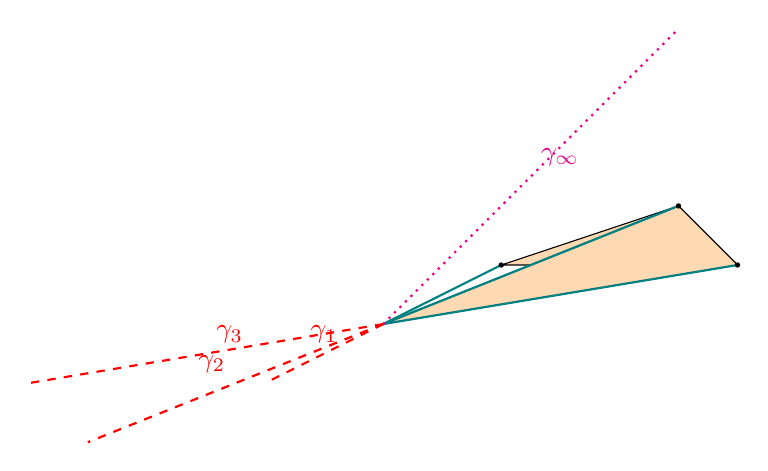
\begin{tikzpicture}[scale=1.5]
    \coordinate (O) at (0,0);
    \coordinate (A) at (1,0.5);
    \coordinate (B) at (2.5,1);
    \coordinate (C) at (3,0.5);

    % Draw the triangles representing the convex hull
    \draw[fill=orange!30] (A) -- (B) -- (C) -- cycle;
    \draw[fill=orange!30] (B) -- (C) -- (O) -- cycle;

    % Draw the coupling vectors (teal)
    \draw[thick, teal] (O) -- (A) node [midway, left] {};
    \draw[thick, teal] (O) -- (B) node [midway, below left] {};
    \draw[thick, teal] (O) -- (C) node [midway, below right] {};

    % Draw the distance vector (purple)
    \draw[dotted, thick, magenta] (O) -- (2.5, 2.5) node [midway, above right] {$\gamma_{\infty}$};

    % Draw the asymptotic vectors (dashed red)
    \draw[dashed, thick, red] (O) -- ($(A)!2!(O)$) node [midway, above] {$\gamma_1$};
    \draw[dashed, thick, red] (O) -- ($(B)!2!(O)$) node [midway, above left] {$\gamma_2$};
    \draw[dashed, thick, red] (O) -- ($(C)!2!(O)$) node [midway, above right] {$\gamma_3$};

    % Label the points
    \draw[fill=black] (A) circle (0.5pt) node [below right] {};
    \draw[fill=black] (B) circle (0.5pt) node [below left] {};
    \draw[fill=black] (C) circle (0.5pt) node [below left] {};

\end{tikzpicture}

\end{document}